\chapter{Analysis}

\section{Backscattered Electron Energy Distribution}
In SEM imaging, we are interested in only the low energy, backscattered electrons. A large percentage of these electrons are secondary/Auger electrons spawned by the higher energy primary electron. As a result, It would be useful to study the energy distribution of the backscattered electrons to better defined the energy threshold for these secondary electrons. In this section, we examine the backscattered electron energy distribution used to produced the image on figure \ref{fig:base}. Also note that since the exact electron generation may be beyond `secondary', it is common for total electron yield to be more than $200\%$. 
\begin{figure}[h]
\begin{center}
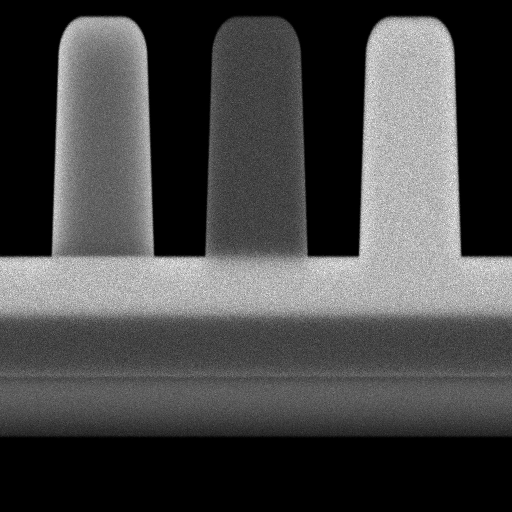
\includegraphics[width=0.5\textwidth]{img/output0.png}
\caption{\label{fig:base}SEM image of a feature with 3 lines}
\end{center}
\end{figure}

The image on figure \ref{fig:base} is generated by with primary electron energy of $1000eV$, beam radius of $0.5nm$ and $200$ electron per location using PMMA, Si and SiO2 as feature materials (left to right) while assume secondary electron energy being below $50eV$. Figure \ref{fig:bse_energy} below shows the energy distribution of backscattered electron at a particular, non--vacuum location on the image. Most of the backscattered electrons detected were low energy electrons, with a small number of of higher energy electrons detected beyond $50eV$. As a result, we conclude that it is safe to categorize electrons with energy lower than $50eV$ as secondary electrons for SEM imaging.
\begin{figure}[h]
\begin{center}
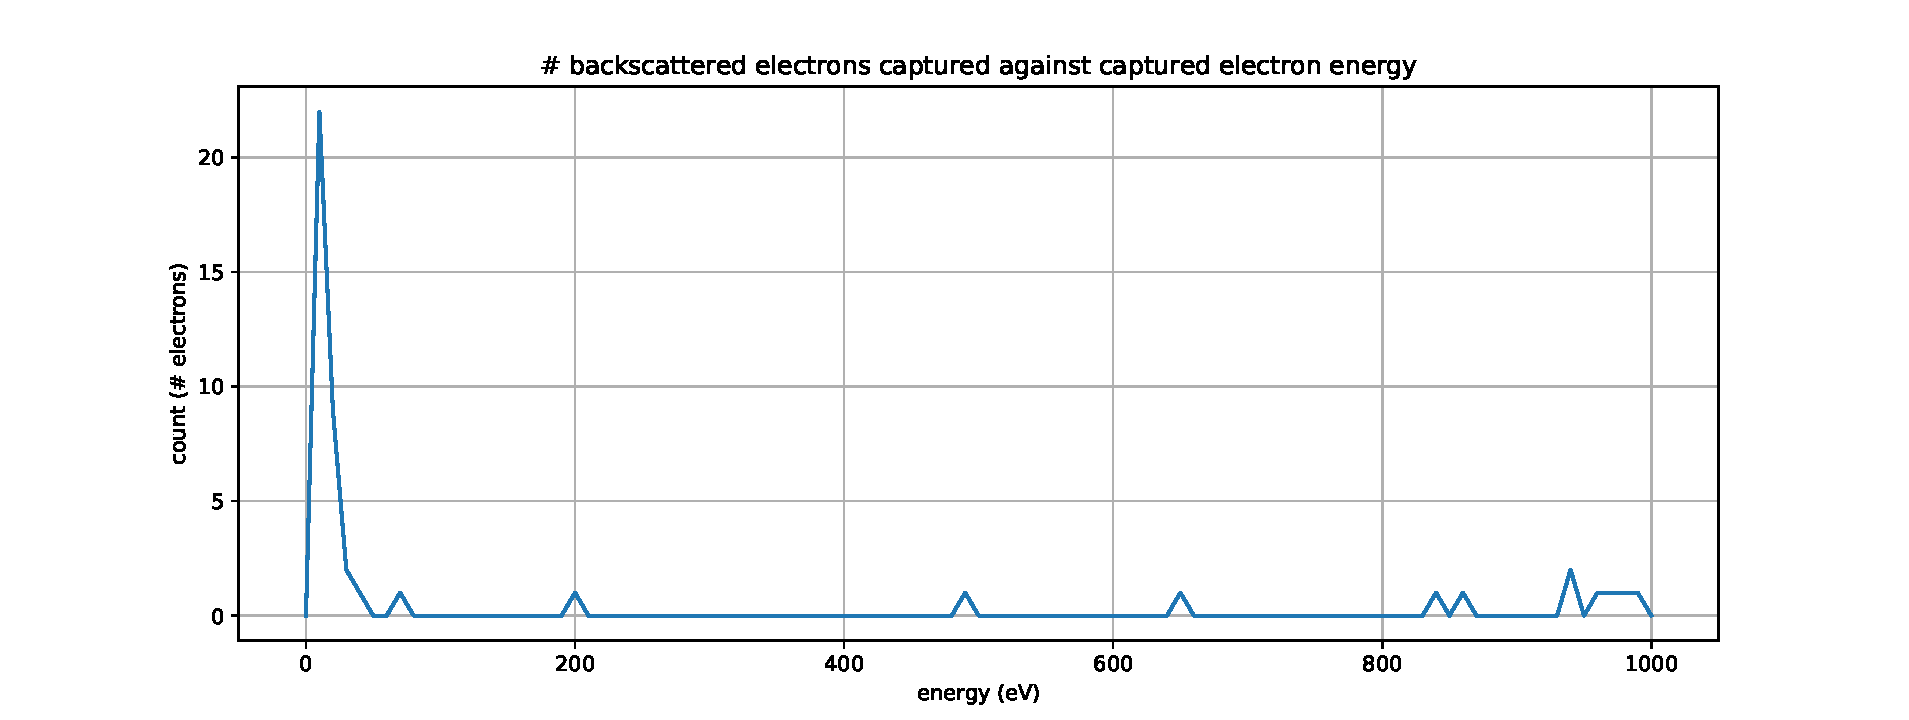
\includegraphics[width=1.0\textwidth]{img/backscattered_energy.pdf}
\caption{\label{fig:bse_energy}Backscattered electron energy distribution on a random, non--vaccum location of the image}
\end{center}
\end{figure}

To show that figure \ref{fig:bse_energy} is a representative energy distribution plot at any non--vacuum location, we produced a heat map of electron energies by acquiring a line scan of non--vacuum locations in figure \ref{fig:bse_heatmap}. The top and bottom rows of figure \ref{fig:bse_heatmap} corresponds to row 16, column 75 and 132 (left and right edges of the feature) on the image \ref{fig:base}. Since similar distributions are observed on different non--vacuum parts of the image, we will assume the distribution in \ref{fig:bse_energy} is a reasonable estimate of the energy distribution at any non--vacuum location.

\begin{figure}[h]
\begin{center}
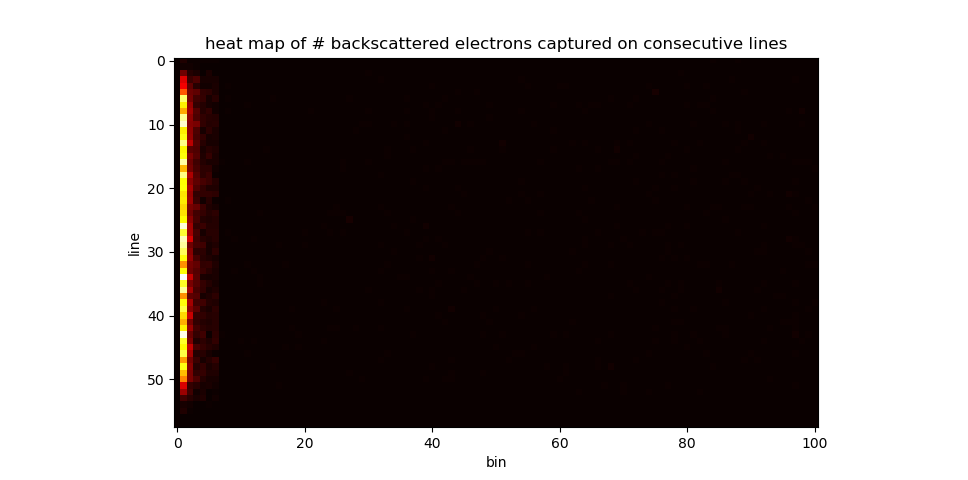
\includegraphics[width=1.0\textwidth]{img/bse_heatmap.png}
\caption{\label{fig:bse_heatmap}Heatmap of backscattered electron energy distribution on a random, non--vacuum line of the image}
\end{center}
\end{figure}

\section{Primary Electron Energy}
In the previous section, we examined the energy distribution of detected electrons and discovered that most detected electrons are SEs with low energy $<50eV$. It would be interesting to find out the effects of different primary electron energy on the SE energy distribution. In this section, we study how the primary electron energy affects the SE yield by comparing the relative quantity of SEs detected when similar electron beams are targetd on three different materials: SiO2, Si, and PMMA.

In this experiment, we used $250$ primary electrons with beam size $.5nm$ and energy of $500eV$ at each location for the first image, and increased the PE energy by $500eV$ for each subsequent image. On every image, there are 3 line features made from PMMA, Si, and SiO2 (left to right), and 3 strips made from SiO2, Si, PMMA (top to down).

\begin{figure}[h]
\begin{center}
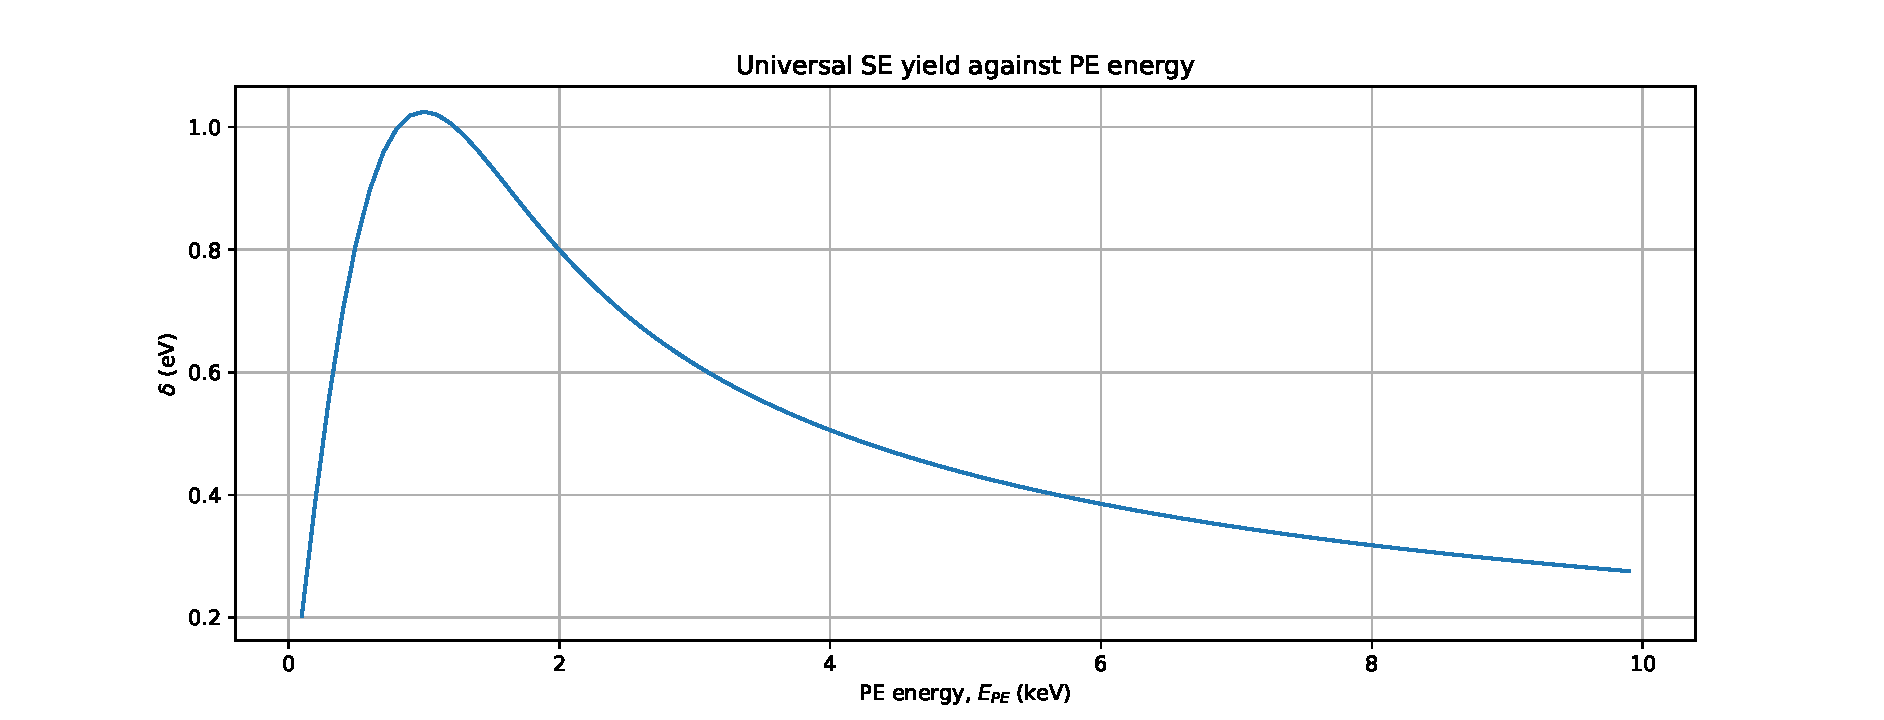
\includegraphics[width=1.0\textwidth]{img/law.pdf}
\caption{\label{fig:se_law}Universal law of SE yield against PE energy\cite{lin_newexam}}
\end{center}
\end{figure}

From the results \ref{fig:diff_beam_energy}, we can clearly see that brightness of all three materials decreased with higher energy. In particular, the relative brightness of Si decreased significantly relative to the other 2 materials, followed by PMMA while that of SiO2 remained approximately the same. The decrease in brightness in all 3 materials is consistent with the ``universal law of SE yield'', given in \cite{lin_newexam} by the equation \ref{eq:se_law} and figure \ref{fig:se_law}

\begin{figure}
\centering
\begin{subfigure}{.5\textwidth}
  \centering
  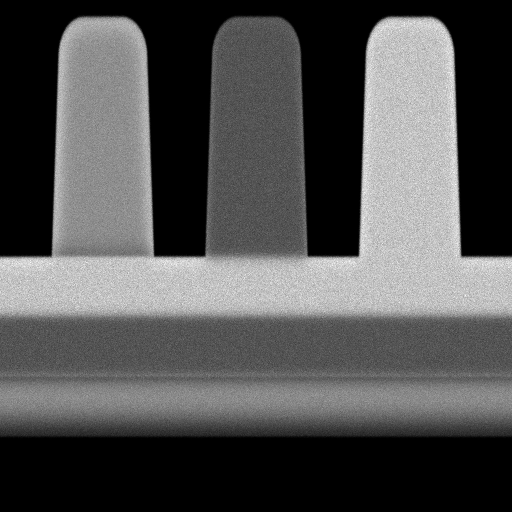
\includegraphics[width=.75\linewidth]{img/500eV.png}
  \caption{500eV beam energy}
  \label{fig:500eV}
\end{subfigure}%
\begin{subfigure}{.5\textwidth}
  \centering
  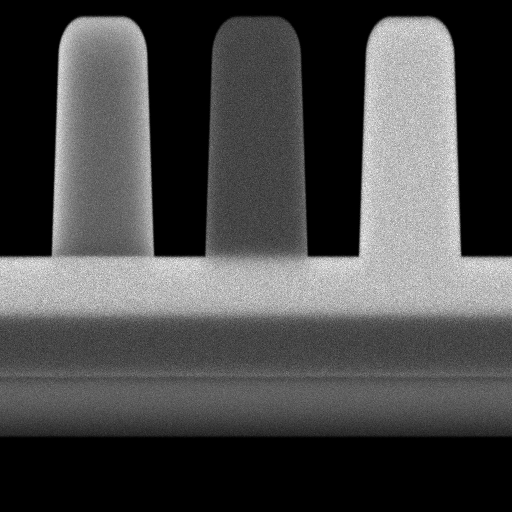
\includegraphics[width=.75\linewidth]{img/1000eV.png}
  \caption{1000eV beam energy}
  \label{fig:1000eV}
\end{subfigure}
\caption{2 images with same setup using different beam energy}
\label{fig:diff_beam_energy}
\end{figure}

\begin{align*}
   \frac{\delta}{\delta^m} &= 1.28\left(\frac{E_{PE}}{E_{PE}^m}\right)^{-0.67}\left(1-exp\left(-1.614\left(\frac{E_{PE}}{E_{PE}^m}\right)^{1.67}\right)\right) \numberthis \label{eq:se_law}
\end{align*}

where $\delta^m$ is the maximum yield, which we assumed to be 1 and $E_{PE}^m \approx 1keV$ is the primary energy of the electron where the maximum is obtained. In particular for Si, the change in brightness shows that its SE yield reaches a maximum at a few hundred electron volts and decreases monotonically at approximately $1/E_{PE}$\cite{lin_newexam} as the energy increases \cite{francesc_conventional}\cite{walker_see}.

\section{Gaussian Beam Radius}
\section{Number of Electron Trajectory per Location}